\documentclass[times, utf8, seminar]{fit}
\usepackage{booktabs}

\begin{document}

\title{Analiza poslovnih podataka sa "open source" software-om}

\author{Ernad Husremović}
\brindex{DL 2792}
\verzija {1.9.0}

\mentor{prof.dr Vanja Bevanda}

\maketitle

\tableofcontents

\chapter{Uvod}

\section{BI Pojmovi}

\subsection{ETL}

Cleansing

\subsection{Mondrian}

Snowflake mondrian - join

\cite{web:pentaho:mondrian_schema}

\subsection{datamart vs datawarehouse}

'Data mart' sadrži informacije o jednom dijelu organizacije (npr. prodaja, ljudski resursi), dok 'datawarehouse' sadrži informacije iz više područja -  obrađuje organizaciju globalno. 

'Data warehouse' je stoga usmjeren na podršku 'top' menadžmenta, dok 'datamart' obezbjeđuje informacije za upravljanje i operativno planiranje pojedinih dijelova organizacije  \cite[str.~391]{pentaho32}.

\subsection{Konstrukcija OLAP kocke}

surogat key (id)

business key (bk)

dimension table

facts table

SCD slow changing dimension
\begin{itemize}
  \item Type I
  \item Type II
\end{itemize}

\begin{figure}
\centering
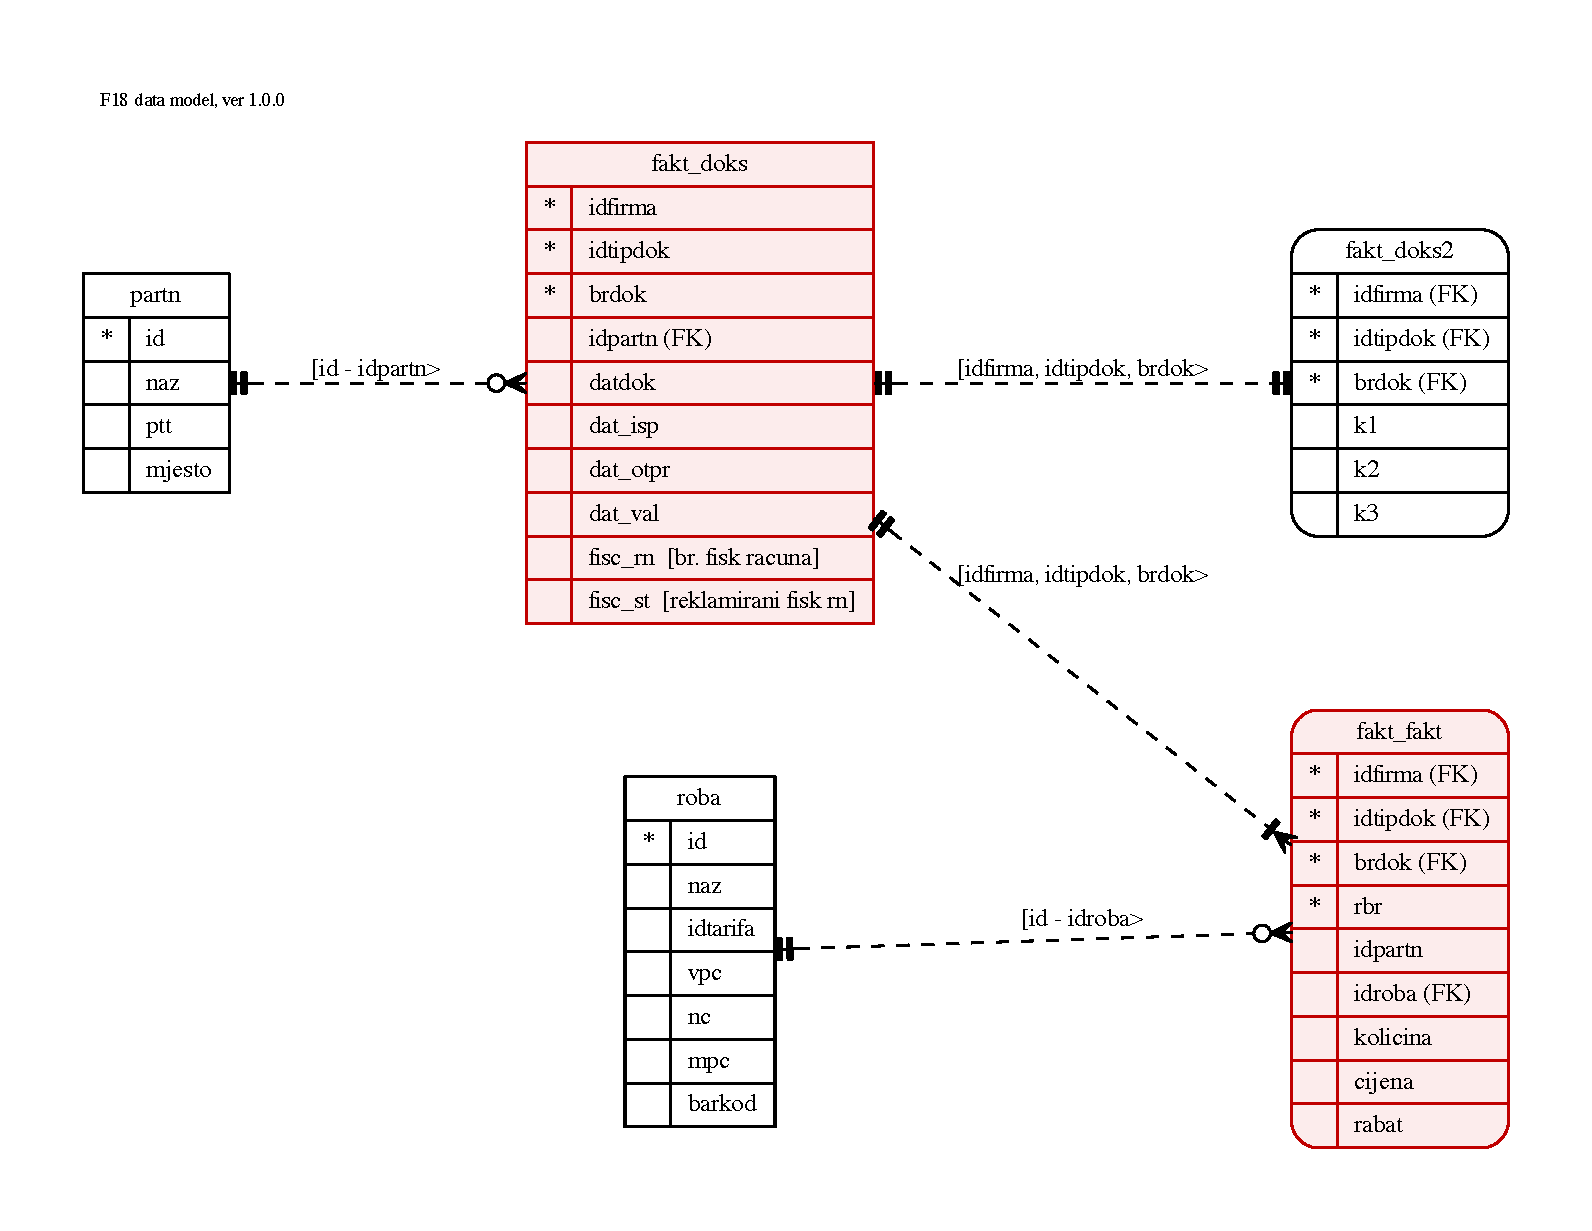
\includegraphics[width=15cm]{img/F18_db.pdf}
\caption{F18 operativni podaci prodaje}
\end{figure}

\section{Pentaho}

Pentaho: analysis multidimensional, reporting, dashboards (key performance indicators) \cite[str.~7]{pentaho32}.

\begin{figure}
\centering
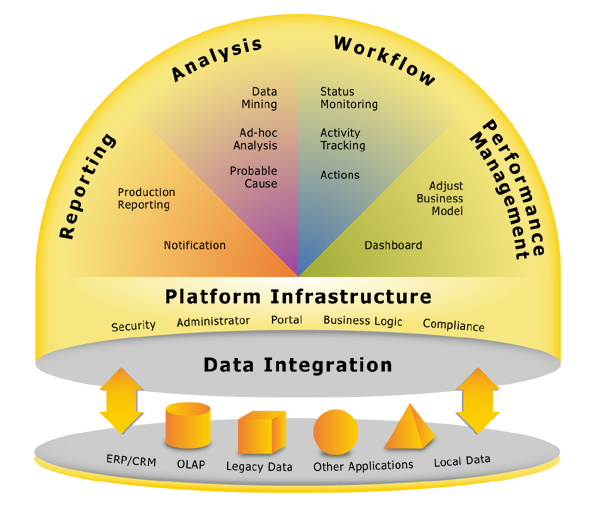
\includegraphics[width=15cm]{img/pentaho_arhitektura_eric.png}
\caption{Pentaho arhitektura (\cite{web:eric})}
\end{figure}



Spoon

data mining weka ?


\subsection{dimension table}

\begin{figure}
\centering
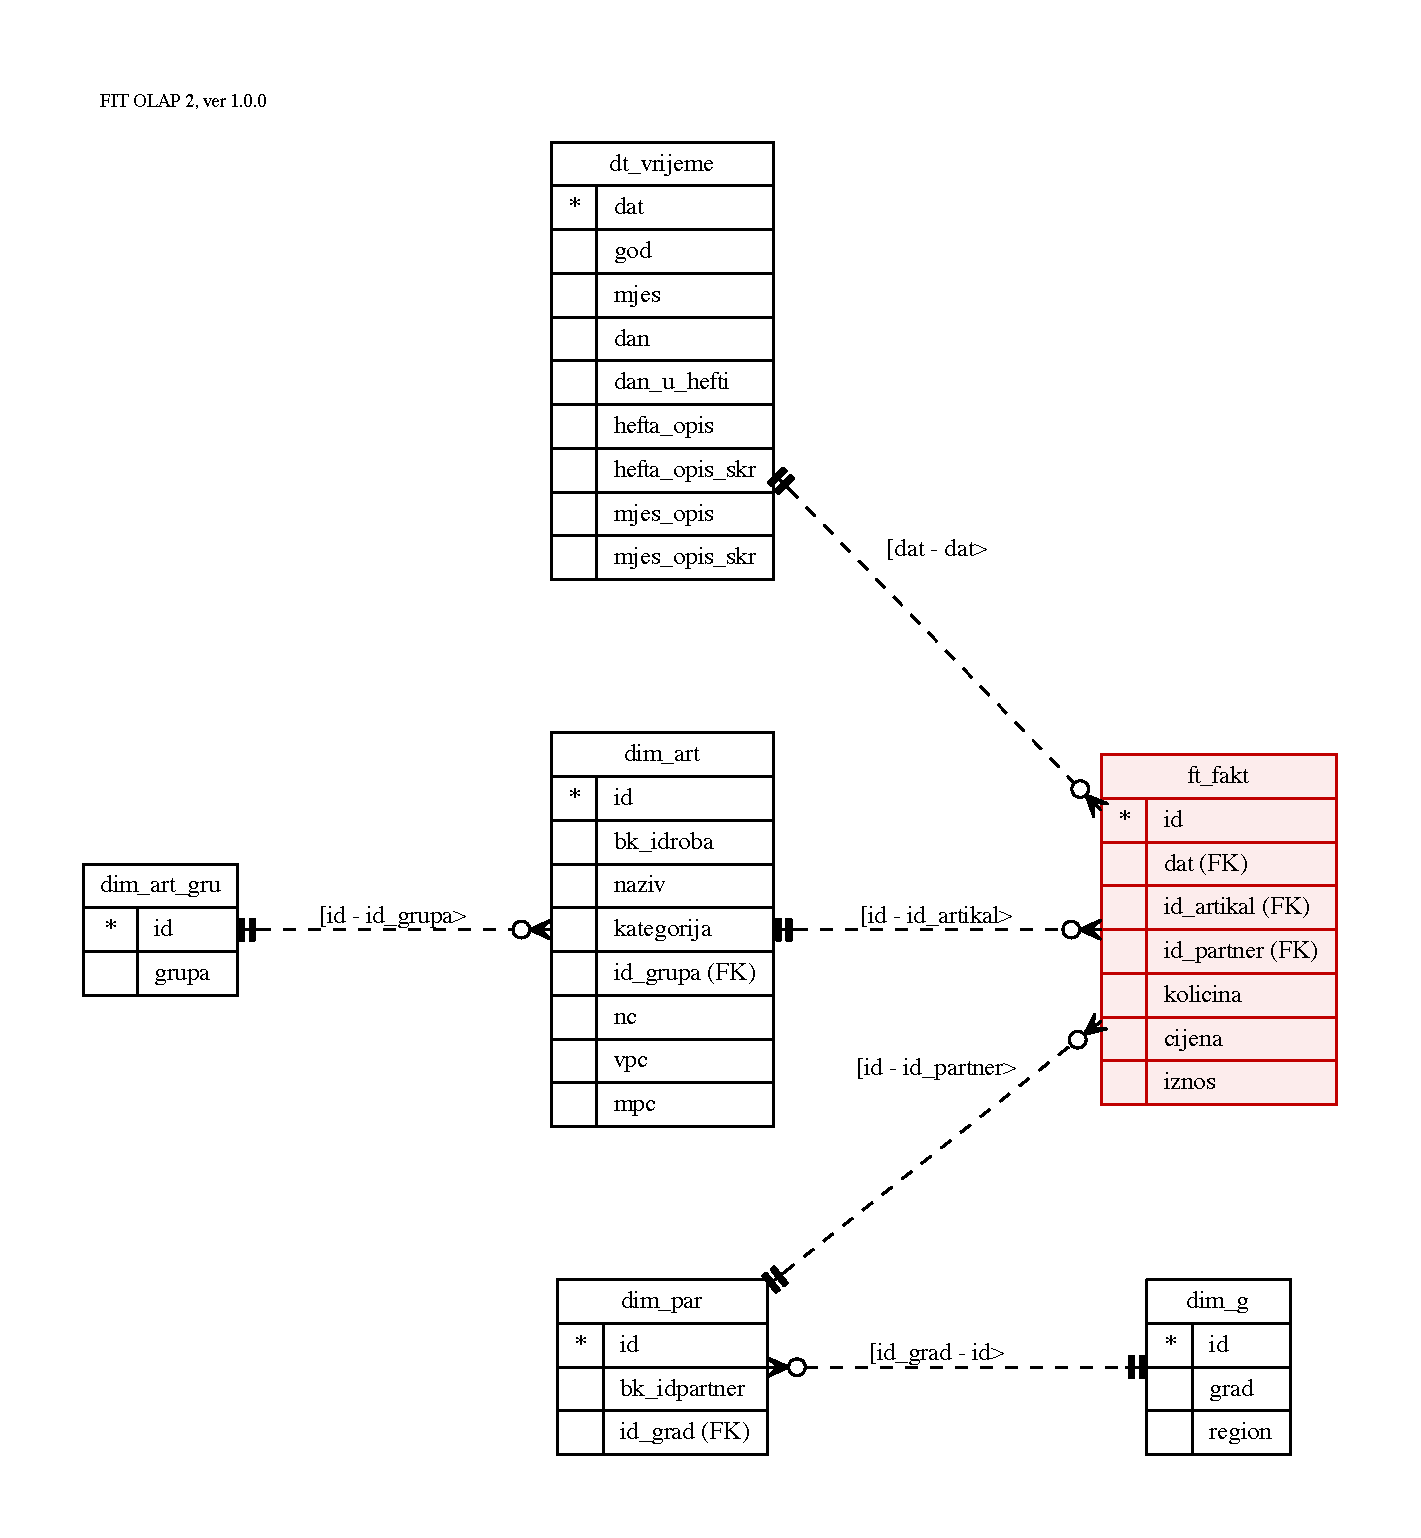
\includegraphics[width=15cm]{img/F18_olap.pdf}
\caption{OLAP schema}
\end{figure}


\subsection{facts table}



\subsection{ETL (Extract Transforn Load)}




\section{Poslovna pitanja (Business questions)}

Kolika je prodaja u određenom vremenskom periodu ?

Kakav je odnos prodaje prodaje za određeni period tekuće godine u odnosu na predhodne ?

Koji su efekti zapošljavanja radnika po pitanju ostvarnih prihoda ?


\subsection{Ekspert}

Poznavanje sadržaja i postojećih struktura podataka.





navodim pentaho: \cite{pentaho32}

navodim stranu 215: \cite[str.~215]{pentaho32}

wikipedia olap cube: \cite{web:wikipedia:olap_cube}
wikipedia xmla: \cite{web:wikipedia:xmla}

\chapter{Zaključak}
Zaključak.

\bibliography{literatura}
\bibliographystyle{fit}

\chapter{Rezime}
Rezime.

\appendix

\chapter{Korišteni alati}

\chapter{Pregled toga i toga}

...


\end{document}
